\chapter{HASIL DAN PEMBAHASAN}

Bab ini menjelaskan uji coba yang dilakukan pada sistem yang telah dibangun beserta analisis dari uji coba yang telah dilakukan. Pembahasan pengujian meliputi lingkungan uji coba, skenario uji coba serta analisis setiap pengujian.

\section{Skenario uji coba}

Subbab ini akan menjelaskan hasil pengujian program penyelesaian permasalahan. Pengujian dilakukan untuk tiga metode: metode repetisi pencarian biner, kode biner, dan kode biner dengan tabel pencarian. Ada dua metode pengujian yang digunakan:

\begin{enumerate}
  \item Pengujian lokal. Pengujian ini menggunakan mesin yang digunakan dalam pemgembang untuk mengukur kebenaran dan informasi hasil query, waktu eksekusi, dan penggunaan memori. Selain itu akan dilakukan pengujian untuk menentukan fungsi seleksi pada algoritma pencarian mendalam dengan pendekatan \textit{greedy}
  \item Pengujian luar. Pengujian ini menggunakan Online Judge untuk mengukur kebenaran dan informasi lain mengenai program.
\end{enumerate}

\section{Lingkungan Uji Coba}

Pengujian dibagi menjadi dua jenis, yaitu dengan dataset buatan dan dengan dataset online. Uji coba dilakukan pada perangkat dengan spesifikasi berikut.

\begin{enumerate}
  \item Perangkat Keras
  \begin{enumerate}
    \item Processor Intel® Core™ i7-7400 CPU @ 3.00GHz (4 CPUs), ~3.0GHz
    \item Random Access Memory 3837MB
  \end{enumerate}
  \item Perangkat Lunak
  \begin{enumerate}
    \item Sistem Operasi Linux Ubuntu 16.04
    \item Bahasa Pemrograman C++
    \item gcc 5.4.0
  \end{enumerate}
  \item Pengujian online SPOJ
  \begin{enumerate}
    \item Time limit: 20s
    \item Source limit: 50000B
    \item Memory limit: 1536MB
    \item Cluster: Cube (Intel G860)
    \item Languages: C++ 4.3.2
  \end{enumerate}
\end{enumerate}

\section{Uji coba menggunakan dataset lokal}

Tahap pengujian adalah melakukan uji coba menggunakan dataset sesuai pada batasan permasalahan untuk mengetahui hasil dan performa dari algoritma dan struktur data yang dibangun. Pengujian juga akan digunakan untuk membandingkan jumlah query, waktu, dan memory dari algoritma dari semua kasus uji dataset. Dataset akan divariasikan sesuai dengan jumlah ruang pencarian $M$ dan jumlah maksimal bohong $e$.

\subsection{Hasil pengujian fungsi seleksi greedy}

Pada pengujian empat fungsi seleksi \textit{gredy}, dataset yang digunakan adalah ruang pencarian $M=2^m \mid 1 \leq m \leq 12$ dan jumlah maksimal bohong $2 \leq e \leq 16$. Hasil yang akan dilihat adalah jumlah query dari setiap fungsi seleksi, semakin sedikit query pada semua kasus uji maka akan semakin bagus. Algoritma \textit{greedy} dengan empat variasi fungsi seleksi akan dibandingkan dengan algoritma repetisi biner \textit{ground truth}. Hasil algoritma repetisi biner juga akan menjadi batas maksimal query, jika jumlah query hasil algoritma \textit{greedy} melebihi jumlah query hasil repetisi biner, maka jumlah query repetisi biner yang akan dipilih.

\begin{figure}
\centering
\begin{tikzpicture}
\begin{axis}[
xlabel={Jumlah maksimal bohong $e$},
ylabel={Jumlah query},
legend pos=north west,
grid style=dashed,
legend entries={1,2,3,4,5},
]
\addplot[green,mark=*] table{data/brute-min.dat};
\addplot[red,mark=o] table{data/brute-min-max.dat};
\addplot[blue,mark=o] table{data/brute-max-min.dat};
\addplot[purple,mark=*] table{data/brute-min-mincount.dat};
\addplot[black,mark=o] table{data/brute-repetition.dat};
\end{axis}
\end{tikzpicture}
\caption{Grafik pengujian fungsi seleksi greedy}
\label{fig:graph_selection_function}
\end{figure}

Pada Gambar \ref{fig:graph_selection_function}, legenda nomor satu sampai lima secara berurutan adalah jarak minimum terbesar, jarak minimum terbesar lalu jarak maximum terkecil, pengurangan jarak maximum dengan jarak minimum terkecil, jarak minimum terbesar lalu jumlah angka memiliki nilai minimum terkecil, dan terakhir algoritma repetisi biner. Dari gambar tersebut dapat disimpulkan bahwa fungsi seleksi yang paling optimal adalah minimum terbesar diikuti dengan jumlah angka memiliki nilai minimum terkecil.

\begin{table}[h!]
\caption{Jumlah query keluaran dari Algoritma \textit{exhaustive search}}
\label{tab:query_count}
\begin{center}
\begin{tabular}{|c|c|c|c|}
\hline
$M$ & jumlah query & $M$ & jumlah query \\
\hline
2 & 1 & 128 & 72 \\
\hline
4 & 3 & 256 & 76 \\
\hline
8 & 7 & 512 & 79 \\
\hline
16 & 15 & 1024 & 81 \\
\hline
32 & 31 & 2048 & 84 \\
\hline
64 & 63 & 4096 & 86 \\
\hline
\end{tabular}
\end{center}
\end{table}

Setelah kandidat fungsi seleksi terpilih, keluaran dari algoritma pencarian mendalam dengan inputan $2 \leq 2^m \leq 4096$ dan $e=16$ akan menghasilkan jumlah query seperti pada Tabel \ref{tab:query_count}. Setiap sejumlah query pada setiap $M$ ini akan menghasilkan $d = 33$ pada $128 \leq M \leq 4096$ atau telah menggunakan semua seed yang berjumlah $M-1$ pada $2 \leq M \leq 64$. Hasil query tersebut akan dimasukkan langsung ke dalam code pada solusi optimal pencarian Ulam non interaktif, pada program utama seperti pada Gambar \ref{fig:sourcecode_lookup}.

\begin{figure}
\centering
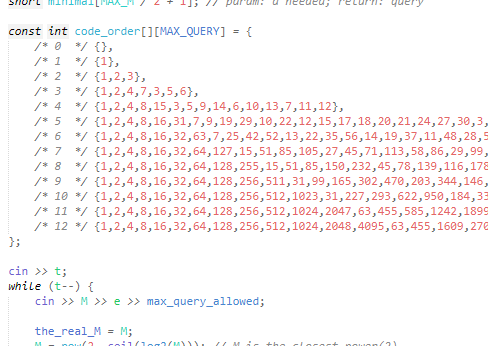
\includegraphics[scale=0.80]{../img/kodingan.png}
\caption{Potongan kode sumber tabel pencarian}
\label{fig:sourcecode_lookup}
\end{figure}

\subsection{Hasil pengujian jumlah query}

Pada pengujian jumlah query, pada setiap ruang pencarian $M=2^m \mid 1 \leq m \leq 12$, pada setiap algoritma, diujikan 15 kasus uji sesuai dengan jumlah maksimal bohong $2 \leq e \leq 16$. Algoritma yang diujikan pada pengujian ini hanya ada dua yaitu algoritma kode biner dan algoritma repetisi biner karena algoritma kode biner dengan tabel pencarian dan algoritma kode biner tanpa tabel pencarian menghasilkan jumlah query yang sama.

Pada Gambar \ref{fig:graph_query1} dapat dilihat bahwa jumlah query yang dihasilkan oleh algoritma kode biner dan repetisi biner sama. Lalu untuk kasus uji selanjutnya, algoritma menunjukkan hasil yang lebih bagus karena menghasilkan jumlah query yang lebih sedikit, seperti yang ditunjukkan pada Gambar \ref{fig:graph_query2}, Gambar \ref{fig:graph_query3}, Gambar \ref{fig:graph_query4}, Gambar \ref{fig:graph_query5}, Gambar \ref{fig:graph_query6}, Gambar \ref{fig:graph_query7}, Gambar \ref{fig:graph_query8}, Gambar \ref{fig:graph_query10}, Gambar \ref{fig:graph_query11}, dan Gambar \ref{fig:graph_query12}. Dari hasil tersebut dapat disimpulkan bahwa algoritma kode biner menghasilkan jumlah query yang lebih sedikit untuk semua $M > 2$ dan untuk semua $e$.

\begin{figure}
\centering
\testgraphquery{1}
\caption{Grafik perbandingan jumlah query pada $M=2$}
\label{fig:graph_query1}
\end{figure}

\begin{figure}
\centering
\testgraphquery{2}
\caption{Grafik perbandingan jumlah query pada $M=4$}
\label{fig:graph_query2}
\end{figure}

\begin{figure}
\centering
\testgraphquery{3}
\caption{Grafik perbandingan jumlah query pada $M=8$}
\label{fig:graph_query3}
\end{figure}

\begin{figure}
\centering
\testgraphquery{4}
\caption{Grafik perbandingan jumlah query pada $M=16$}
\label{fig:graph_query4}
\end{figure}

\begin{figure}
\centering
\testgraphquery{5}
\caption{Grafik perbandingan jumlah query pada $M=32$}
\label{fig:graph_query5}
\end{figure}

\begin{figure}
\centering
\testgraphquery{6}
\caption{Grafik perbandingan jumlah query pada $M=64$}
\label{fig:graph_query6}
\end{figure}

\begin{figure}
\centering
\testgraphquery{7}
\caption{Grafik perbandingan jumlah query pada $M=128$}
\label{fig:graph_query7}
\end{figure}

\begin{figure}
\centering
\testgraphquery{8}
\caption{Grafik perbandingan jumlah query pada $M=256$}
\label{fig:graph_query8}
\end{figure}

% \begin{figure}
% \centering
% \testgraphquery{9}
% \caption{Grafik perbandingan jumlah query pada $M=512$}
% \label{fig:graph_query9}
% \end{figure}

\begin{figure}
\centering
\testgraphquery{10}
\caption{Grafik perbandingan jumlah query pada $M=1024$}
\label{fig:graph_query10}
\end{figure}

\begin{figure}
\centering
\testgraphquery{11}
\caption{Grafik perbandingan jumlah query pada $M=2048$}
\label{fig:graph_query11}
\end{figure}

\begin{figure}
\centering
\testgraphquery{12}
\caption{Grafik perbandingan jumlah query pada $M=4096$}
\label{fig:graph_query12}
\end{figure}

\subsection{Hasil pengujian waktu eksekusi}

Pada pengujian waktu eksekusi, pada setiap algoritma, diujikan 12 kasus uji sesuai dengan jumlah variasi ruang pencarian $M = 2^m \mid 1 \leq m \leq 12$. Pada setiap pengujian, terdapat 15 kasus uji sesuai dengan variasi jumlah maksimal bohong $2 \leq e \leq 16$. Hasil pengujian ditunjukkan pada Gambar \ref{fig:graph_time}, dapat disimpulkan bahwa algoritma kode biner tanpa tabel pencarian menghasilkan laju peningkatan waktu yang tinggi, sedangkan untuk repetisi biner dan kode biner dengan tabel pencarian menghasilkan waktu yang stabil. Hal ini dikarenakan algoritma kode biner tanpa tabel pencarian memiliki kompleksitas $O(M^3)$ pada proses pencarian mendalam, sedangkan pada algoritma kode biner dengan tabel pencarian memiliki kompleksitas $O(1)$ karena proses pencarian mendalam dilakukan sebagai pra proses.

\begin{figure}
\centering
\begin{tikzpicture}
\begin{axis}[
xlabel={Jumlah ruang pencarian($2^m$)},
ylabel={Waktu eksekusi(detik)},
legend pos=north west,
grid style=dashed,
legend entries={Pengulangan biner,Kode biner,Tabel pencarian},
]
\addplot[blue,mark=triangle] table{data/timeR.dat};
\addplot[red,mark=*] table{data/timeB.dat};
\addplot[green,mark=square] table{data/timeL.dat};
\end{axis}
\end{tikzpicture}
\caption{Grafik perbandingan waktu eksekusi}
\label{fig:graph_time}
\end{figure}

\subsection{Hasil pengujian penggunaan memori}

Pada pengujian penggunaan memori, pada setiap algoritma, diujikan 12 kasus uji sesuai dengan jumlah variasi ruang pencarian $1 \leq m \leq 12$. Pada setiap pengujian, terdapat 15 kasus uji sesuai dengan variasi jumlah maksimal bohong $2 \leq e \leq 16$. Hasil pengujian ditunjukkan pada Gambar \ref{fig:graph_time}, terlihat bahwa algoritma kode biner tanpa tabel pencarian menghasilkan laju peningkatan penggunaan memori yang tinggi, sedangkan untuk repetisi biner dan kode biner dengan tabel pencarian menghasilkan penggunaan memori yang stabil, namun algoritma repetisi biner menunjukkan penggunaan memori yang lebih sedikit.

\begin{figure}
\centering
\begin{tikzpicture}
\begin{axis}[
xlabel={Jumlah ruang pencarian($2^m$)},
ylabel={Penggunaan memory(byte)},
legend pos=north west,
grid style=dashed,
legend entries={Pengulangan biner,Kode biner,Lookup table},
]
\addplot[blue,mark=triangle] table{data/memoryR.dat};
\addplot[red,mark=*] table{data/memoryB.dat};
\addplot[green,mark=square] table{data/memoryL.dat};
\end{axis}
\end{tikzpicture}
\caption{Grafik perbandingan penggunaan memory}
\label{fig:graph_memory}
\end{figure}

\section{Uji coba menggunakan dataset online SPOJ}

Selain dataset buatan, program juga akan diuji dengan dataset pada Online Judge SPOJ GUESSN5. Hal yang dinilai pada pengujian adalah banyaknya query yang dibuat, waktu yang dibutuhkan, dan penggunaan memory. Pada pengujian online SPOJ terdapat 30 dataset, yaitu 15 dataset dengan 30 kasus uji dan 15 dataset dengan 99 kasus uji dengan persebaran ruang pencarian $2 \leq M \leq 4096$ dan maksimal bohong $2 \leq e \leq 16$.

Pembobotan skor adalah jika penjawab menemukan ada suatu set jawaban yang menyebabkan lebih dari satu kemungkinan nilai $x$, maka pengujian dianggap gagal. Jika berhasil, maka nilai skor bertambah $q^2$. Jika gagal, maka nilai skor bertambah $4m^2$. Total skor adalah jumlah semua skor dari setiap kasus uji. Semakin kecil skor maka semakin baik algoritma yang digunakan. Skor akan dibandingkan dengan pengajuan peserta lain pada SPOJ GUESSN5. Subbab ini akan menjelaskan hasil pengujian program penyelesaian permasalahan menggunakan algoritma repetisi pencarian biner dan kode biner.

\subsection{Uji coba algoritma repetisi pencarian biner pada SPOJ}

Algoritma repetisi pencarian biner disubmit ke SPOJ dalam bahasa C, menghasilkan penilaian yang ditunjukkan pada Tabel \ref{tab:score_repetitive}. Karena ini adalah algoritma yang pasti benar dengan cara termudah, maka dapat diasumsikan bahwa skor yang didapat dari algoritma ini adalah skor minimal yang dapat menjadi tolok ukur keberhasilan algoritma yang lain.

\begin{table}[h!]
\caption{Hasil algoritma repetisi pencarian biner pada SPOJ}
\label{tab:score_repetitive}
\begin{center}
\begin{tabular} {|l|l|}
\hline
ID & 20152331 \\ \hline
Tanggal & 2017-09-14 06:08:19 \\ \hline
Skor & 42,787,090 \\ \hline
Waktu & 0.00 \\ \hline
Memori & 2.7M \\ \hline
\end{tabular}
\end{center}
\end{table}

\subsection{Uji coba algoritma kode biner pada SPOJ}

Algoritma repetisi pencarian biner disubmit ke SPOJ dalam bahasa C, menghasilkan penilaian yang ditunjukkan pada Tabel \ref{tab:score_brute_binary_code}. Algoritma ini menghasilkan error SIGSEGV karena penggunaan memori melewati batas yang disediakan oleh SPOJ.

\begin{table}[h!]
\caption{Hasil algoritma kode biner pada SPOJ}
\label{tab:score_brute_binary_code}
\begin{center}
\begin{tabular} {|l|l|}
\hline
ID & 21726709 \\ \hline
Tanggal & 2018-05-26 01:10:34 \\ \hline
Skor & runtime error (SIGSEGV) \\ \hline
Waktu & 0.00 \\ \hline
Memori & 3.1M \\ \hline
\end{tabular}
\end{center}
\end{table}

\subsection{Uji coba algoritma kode biner dengan tabel pencarian pada SPOJ}

Algoritma repetisi pencarian biner dengan tabel pencarian disubmit ke SPOJ dalam bahasa C, menghasilkan penilaian yang ditunjukkan pada Tabel \ref{tab:score_binary_code}. Skor ini menjadi skor tertinggi pada SPOJ GUESSN5 seperti yang ditunjukkan pada Gambar \ref{fig:rank_guessn5_spoj}.

\begin{table}[h!]
\caption{Hasil algoritma kode biner pada SPOJ}
\label{tab:score_binary_code}
\begin{center}
\begin{tabular} {|l|l|}
\hline
ID & 21732463 \\ \hline
Tanggal & 2018-05-27 00:45:01 \\ \hline
Skor & 4,225,555 \\ \hline
Waktu & 0.44 \\ \hline
Memori & 2.8M \\ \hline
\end{tabular}
\end{center}
\end{table}

\begin{figure}
\centering
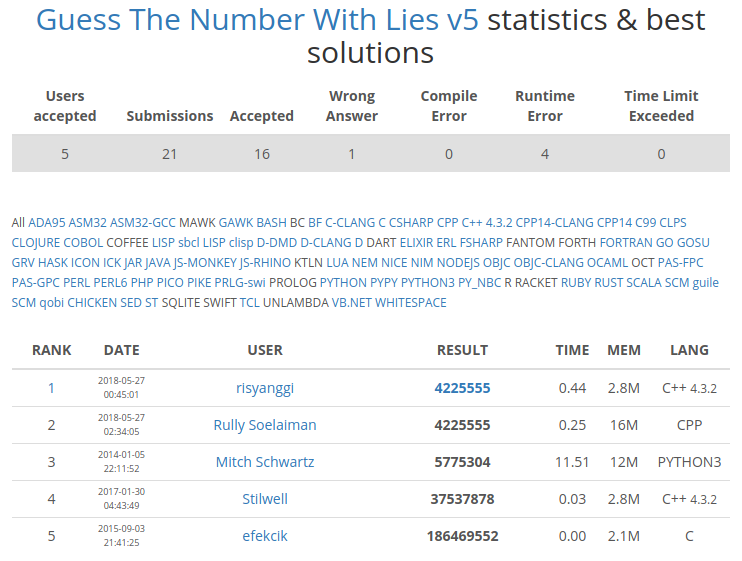
\includegraphics[scale=0.60]{../img/spoj.png}
\caption{Urutan ranking solusi permasalahan GUESSN5 pada SPOJ}
\label{fig:rank_guessn5_spoj}
\end{figure}
